% !TEX root = main.tex
\section{Obecny stan i dalszy rozwój narzędzia GenericMonitoringTool}
Narzędzie GenericMonitoringTool staje się chętnie wykorzystywanym rozwiązaniem w ramach platformy Athena, na potrzeby tworzenia histogramów i monitorowania kodu.
W momencie pisania tej pracy, w jej kodzie zadeklarowanych jest ponad 450 zmiennych monitorowanych w obrębie 53 różnych algorytmów. 
Mogą one wypełnić danymi prawie 4500 zdefiniowanych histogramów.

\subsection{Zastosowanie w systemie wyzwalania online}
Pierwotnie GenericMonitoringTool był tworzony z myślą o użyciu go w systemie wyzwalania online i to w tym obszarze jest najczęściej wykorzystywany~\cite{online-monitoring-guide}. 
Dla tego rodzaju użycia, szybkość działania jest jedną z kluczowych cech. 
Było to powodem przeprowadzenia testów wydajnościowych opisanych w rozdziale \ref{generic-monitoring-tool-description}.

GenericMonitoringTool został szeroko wykorzystany podczas technicznego "reprocessingu" dla 22 wersji platformy Athena, dla którego przykładowe histogramy zostały przedstawione na rysunkach~\ref{fig:athena:histogram_TH1},~\ref{fig:athena:histogram_TH1_time},~\ref{fig:athena:histogram_TH2}.
Konfigurację, w której zadeklarowano te histogramy przedstawiono na listingu~\ref{lst:athena:histogram_declaration}. W liniach 7, 9 i 11 użyto metodę pomocniczą `defineHistogram`, która upraszcza i systematyzuje proces deklaracji histogramu w ramach narzędzia GenericMonitoringTool. To w tych liniach określone zostały: nazwy zmiennych monitorowanych, typ histogramu, ścieżka gdzie zostanie zachowany histogram, jego tytuł, oraz zakresy wartości na poszczególnych osiach.
Natomiast na listingach~\ref{lst:athena:track_pt},~\ref{lst:athena:time_calibration_streamer},~\ref{lst:athena:track_eta_vs_track_phi}, dołączone zostały odpowiadające fragmenty kodu C++, odpowiedzialnego za stworzenie zmiennych i grup monitorowanych oraz wypełnienie ich danymi.

I tak zmienna monitorowana, poprzeczny pęd śladu (w praktyce pęd $\times$ ładunek) jest deklarowana jako skalar - listing~\ref{lst:athena:track_pt}, linia 6. 
Następnie definiowana jest grupa monitorowana, w której wraz z tą zmienna, definiowane są inne parametry śladu muonów (np. kąty emisji czy ilości sygnałów w detektorze, które użyte zostały w rekonstrukcji) znalezionych przez szybki algorytm rekonstrukcji używany online - linia 8. 
Kolejnym krokiem jest przypisanie wartości do tej zmiennej, które jest zrealizowane w linii 10.
Opcjonalną operacją jest użycie zmiennej monitorowanej jako zwykłej wartości liczbowej `double`- przedstawione w linii 11.

Listing~\ref{lst:athena:time_calibration_streamer} prezentuje monitorowanie czasu wykonania algorytmu poprzez użycie klasy Monitored::Timer - linia 10. 
Podobnie jak w przypadku zmiennej typu skalar, do poprawnego działania niezbędne jest stworzenie grupy monitorowanej - linia 12.
Kolejnym krokiem jest uruchomienie `timera` poprzez wywołanie metody `start()` w linii 14.
Następnie wykonywane są operacje, których czas wykonania chcemy zmierzyć; w tym wypadku jest to wywołanie metody `createRoiFragment` - linia 16.
Ostatnią akcją jest wywołanie metody `stop()` na obiekcie `timer`, które kończy pomiar czasu - linia 18.

Listing~\ref{lst:athena:track_eta_vs_track_phi} przedstawia proces wypełnienia histogramu 2D z użyciem monitorowanych kolekcji.
W liniach 6, 8, 9 przygotowywane są 2 zmienne typu `std::vector<float>`, które następnie przekazywane są do monitorowania w liniach 11 i 12.
Tak samo jak w przypadku zmiennej typu skalar i `timer`, niezbędne jest zadeklarowanie grupy monitorowanej zawierającej te zmienne - linia 14.
Kolejnym krokiem jest wypełnienie przygotowanych kolekcji danymi; realizowane jest to w liniach 17 i 18. 
W przeciwieństwie do zmiennej typu skalar, kod nie operuje na typie monitorowanym `Monitored::Collection`. 
Danymi wypełniane są pierwotnie zadeklarowane kolekcje `std::vector<float>` i to ich zawartość zostanie użyta do wypełnienia histogramu.

We wszystkich powyższych przykładach, wartości zmiennych monitorowanych zostaną wpisane do histogramów, w momencie wywołania destruktora obiektu `Monitored::Group`.

\begin{figure}[!ht]
\centering
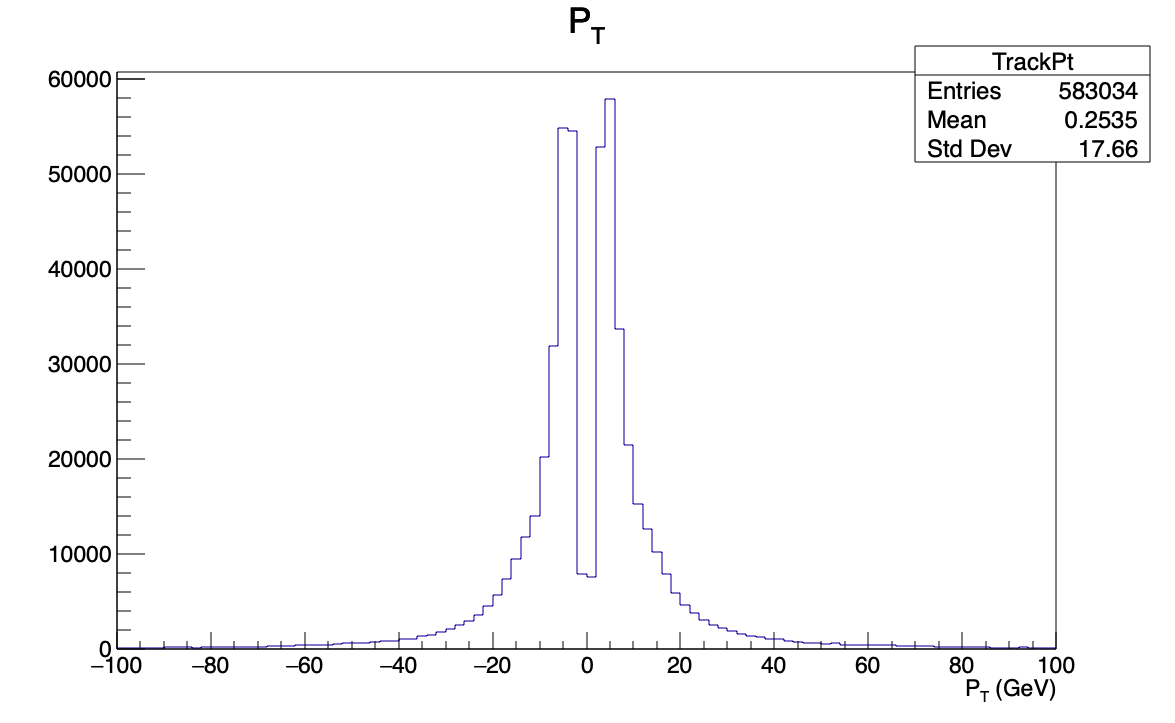
\includegraphics[width=1\textwidth]{img/histogram_TH1.png}
\caption{
Histogram TH1F dla zmiennej monitorowanej typu 'Scalar', utworzony z pomocą GenericMonitoringTool. Powstał podczas technicznego "reprocessingu" 22 wersji platformy Athena.
}
\label{fig:athena:histogram_TH1}
\end{figure}

\begin{figure}[!ht]
\centering
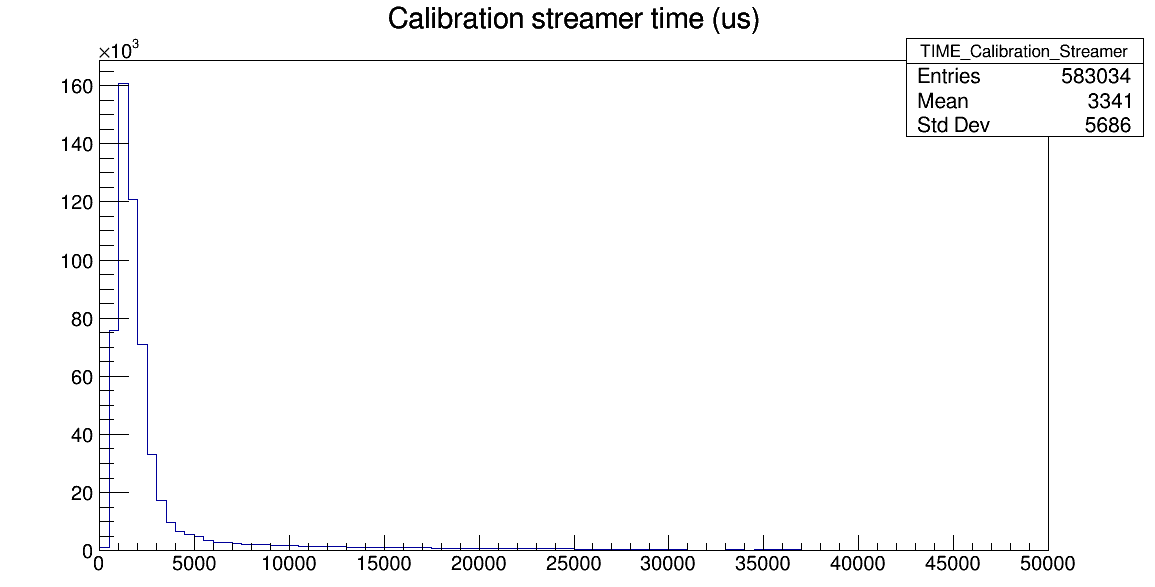
\includegraphics[width=1\textwidth]{img/histogram_TH1_time.png}
\caption{
Histogram TH1F dla zmiennej monitorowanej typu 'Timer', utworzony z pomocą GenericMonitoringTool. Powstał podczas technicznego "reprocessingu" 22 wersji platformy Athena.
}
\label{fig:athena:histogram_TH1_time}
\end{figure}

\begin{figure}[!ht]
\centering
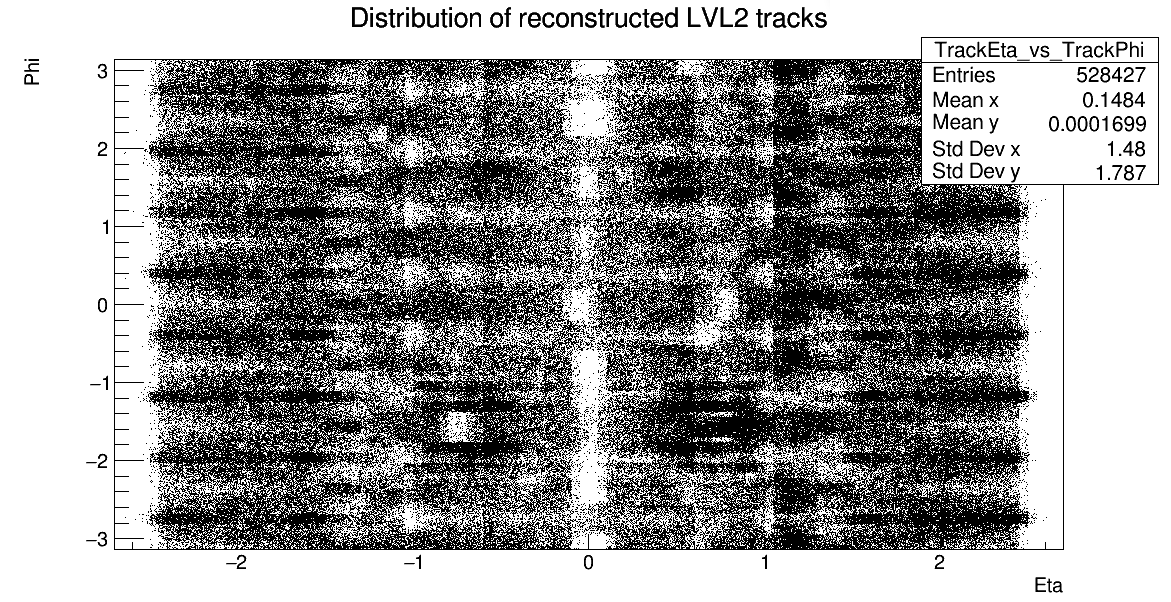
\includegraphics[width=1\textwidth]{img/histogram_TH2.png}
\caption{
Histogram TH2F dla dwóch zmiennych monitorowanych typu 'Collection', utworzony z pomocą GenericMonitoringTool. Powstał podczas technicznego "reprocessingu" 22 wersji platformy Athena.
}
\label{fig:athena:histogram_TH2}
\end{figure}

\FloatBarrier

\begin{python}[caption={Fragment kodu konfiguracji Athena Python~\cite{histogram-declaration}, zawierającego deklarację histogramów przedstawionych na rysunkach~\ref{fig:athena:histogram_TH1},~\ref{fig:athena:histogram_TH1_time}~i~\ref{fig:athena:histogram_TH2}.}, label={lst:athena:histogram_declaration}]
class TrigL2MuonSAMonitoring(GenericMonitoringTool):
    def __init__ (self, name = "TrigL2MuonSAMonitoring"):
        super(TrigL2MuonSAMonitoring, self).__init__( name )
    
        self.HistPath = name
(*@\centerline{\raisebox{-1pt}[0pt][0pt]{$\vdots$}}@*)
        self.defineHistogram('TrackPt', type='TH1F', path='EXPERT', title="P_{T};P_{T} (GeV)", xbins=100, xmin=-100, xmax=100 )
(*@\centerline{\raisebox{-1pt}[0pt][0pt]{$\vdots$}}@*)
        self.defineHistogram('TrackEta, TrackPhi', type='TH2F', path='EXPERT', title="Distribution of reconstructed LVL2 tracks; Eta; Phi", xbins=108, xmin=-2.7, xmax=2.7, ybins=96, ymin=-3.1416, ymax=3.1416 )
(*@\centerline{\raisebox{-1pt}[0pt][0pt]{$\vdots$}}@*)
        self.defineHistogram('TIME_Calibration_Streamer', type='TH1F', path='EXPERT', title="Calibration streamer time (us)", xbins=100, xmin=0, xmax=50000 )
\end{python}

\begin{cpp}[caption={Fragment kodu algorytmu~\cite{histogram-fill}, odpowiadającego za wypełnienie histogramu przedstawionego na rysunku~\ref{fig:athena:histogram_TH1}, za pomocą zmiennej monitorowanej `TrackPt`.}, label={lst:athena:track_pt}]
StatusCode MuFastSteering::updateMonitor(const LVL1::RecMuonRoI* roi,
  const TrigL2MuonSA::MdtHits& mdtHits,
  std::vector<TrigL2MuonSA::TrackPattern>& trackPatterns)
{
(*@\centerline{\raisebox{-1pt}[0pt][0pt]{$\vdots$}}@*)
  auto track_pt 	= Monitored::Scalar("TrackPt", 9999.);
(*@\centerline{\raisebox{-1pt}[0pt][0pt]{$\vdots$}}@*)
  auto monitorIt	= Monitored::Group(m_monTool, inner_mdt_hits, middle_mdt_hits, outer_mdt_hits, invalid_rpc_roi_number, efficiency, sag_inverse, address, absolute_pt, sagitta, track_pt, track_eta, track_phi, failed_eta, failed_phi, res_inner, res_middle, res_outer, fit_residuals);
(*@\centerline{\raisebox{-1pt}[0pt][0pt]{$\vdots$}}@*)
  track_pt = (fabs(pattern.pt ) > ZERO_LIMIT) ? pattern.charge*pattern.pt : 9999.;
  absolute_pt = fabs(track_pt);
(*@\centerline{\raisebox{-1pt}[0pt][0pt]{$\vdots$}}@*)
}
\end{cpp}

\begin{cpp}[caption={Fragment kodu algorytmu~\cite{histogram-fill}, odpowiadającego za wypełnienie histogramu przedstawionego na rysunku~\ref{fig:athena:histogram_TH1_time}, za pomocą zmiennej monitorowanej `TIME\_Calibration\_Streamer`.}, label={lst:athena:time_calibration_streamer}]
StatusCode MuFastSteering::findMuonSignature(
  const DataVector<const TrigRoiDescriptor>& roids,
  const DataVector<const LVL1::RecMuonRoI>& muonRoIs,
  DataVector<xAOD::L2StandAloneMuon>& outputTracks,
  TrigRoiDescriptorCollection& outputID,
  TrigRoiDescriptorCollection& outputMS,
  DataVector<xAOD::TrigComposite>& outputComposite)
{
(*@\centerline{\raisebox{-1pt}[0pt][0pt]{$\vdots$}}@*)
  auto calibrationTimer = Monitored::Timer("TIME_Calibration_Streamer");

  auto monitorIt	= Monitored::Group(m_monTool, prepTimer, patternTimer, stationFitterTimer, trackFitterTimer, trackExtraTimer, calibrationTimer);
(*@\centerline{\raisebox{-1pt}[0pt][0pt]{$\vdots$}}@*)
  calibrationTimer.start();
(*@\centerline{\raisebox{-1pt}[0pt][0pt]{$\vdots$}}@*)
  sc = m_calStreamer->createRoiFragment(*p_roi,tp,m_mdtHits_normal, m_rpcHits, m_tgcHits, m_calBufferSize, m_calDataScouting, updateTriggerElement); 
(*@\centerline{\raisebox{-1pt}[0pt][0pt]{$\vdots$}}@*)
  calibrationTimer.stop();
(*@\centerline{\raisebox{-1pt}[0pt][0pt]{$\vdots$}}@*)
}
\end{cpp}

\begin{cpp}[caption={Fragment kodu algorytmu~\cite{histogram-fill}, odpowiadającego za wypełnienie histogramu przedstawionego na rysunku~\ref{fig:athena:histogram_TH2}, za pomocą monitorowanych kolekcji `TrackEta` oraz `TrackPhi`.}, label={lst:athena:track_eta_vs_track_phi}]
StatusCode MuFastSteering::updateMonitor(const LVL1::RecMuonRoI* roi,
  const TrigL2MuonSA::MdtHits& mdtHits,
  std::vector<TrigL2MuonSA::TrackPattern>& trackPatterns)
{
(*@\centerline{\raisebox{-1pt}[0pt][0pt]{$\vdots$}}@*)
  std::vector<float> t_eta, t_phi;
(*@\centerline{\raisebox{-1pt}[0pt][0pt]{$\vdots$}}@*)
  t_eta.clear();
  t_phi.clear();
(*@\centerline{\raisebox{-1pt}[0pt][0pt]{$\vdots$}}@*)
  auto track_eta	= Monitored::Collection("TrackEta", t_eta);
  auto track_phi	= Monitored::Collection("TrackPhi", t_phi);
(*@\centerline{\raisebox{-1pt}[0pt][0pt]{$\vdots$}}@*)
  auto monitorIt	= Monitored::Group(m_monTool, inner_mdt_hits, middle_mdt_hits, outer_mdt_hits, invalid_rpc_roi_number, efficiency, sag_inverse, address, absolute_pt, sagitta, track_pt, track_eta, track_phi, failed_eta, failed_phi, res_inner, res_middle, res_outer, fit_residuals );
(*@\centerline{\raisebox{-1pt}[0pt][0pt]{$\vdots$}}@*)
  if (fabs(pattern.etaMap) > ZERO_LIMIT || fabs(pattern.phiMS) > ZERO_LIMIT) {
    t_eta.push_back(pattern.etaMap);
    t_phi.push_back(pattern.phiMS);
  }
(*@\centerline{\raisebox{-1pt}[0pt][0pt]{$\vdots$}}@*)
}
\end{cpp}

\subsection{Zastosowanie do monitorowania offline - Data Quality}
GenericMonitoringTool jest obecnie głównym narzędziem wykorzystywanym do monitorowania jakości danych (Data Quality) offline~\cite{atlas-multithread-article}.
Ze względu na nieco inne zastosowanie, użyte są dodatkowe klasy algorytmów DQ, a odwołania do narzędzia GMT są nieco bardziej ukryte.
Rysunek~\ref{fig:athena:offlineDiagram} pokazuje zależności między klasami w środowisku DQ.
Obecnie, dodawane są także nowe funkcjonalności pozwalające na pokrycie większej ilości przypadków użycia.

\begin{figure}[!ht]
\centering
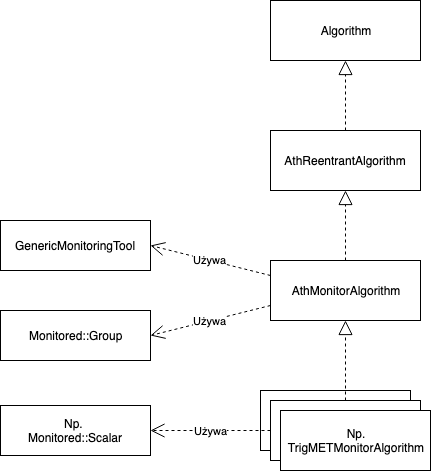
\includegraphics[width=0.75\textwidth]{img/offline_diagram.png}
\caption{
Zależności pomiędzy klasami w środowisku DQ offline.
}
\label{fig:athena:offlineDiagram}
\end{figure}

Listing~\ref{lst:athena:dq_histogram_declaration} pokazuje konfigurację GMT dla histogramów monitorujących brakujące energie, np. neutrin lub innych nie oddziaływujących cząstek.
Pozwala to na monitorowanie jakości danych zbieranych przez linie trygera, wyszukującą takie właśnie przypadki.
W systemie offline DQ histogramy są wstępnie kategoryzowane jako te do automatycznego sprawdzenia (Shifter), lub przeznaczone dla ekspertów (Expert).
Dla każdej z tych grup są one definiowane niezależnie. 

Listing~\ref{lst:athena:dq_histogram_fill} prezentuje proces wypełnienia histogramów DQ danymi.
Podobnie jak w przypadku histogramów online, używane są tu zmienne monitorowane typu skalar - linie 1-9. 
Taki sam jest również proces przypisywania do nich wartości - linie 11-23.
Różni się natomiast sposób dostępu do grup monitorowanych - linie 25-28.
Wykorzystywane są tu metody pomocnicze `fill()` oraz `getGroup()`, zdefiniowane w klasie `AthMonitorAlgorithm`.
Ich wewnętrzna implementacja wykorzystuje grupy monitorowane.
Są one więc interfejsem ukrywającym przed użytkownikiem instancje GMT, odpowiednio skonfigurowane, tak aby wypełniać właściwe histogramy - najczęściej będące podzbiorem wszystkich możliwych do wytworzenia. 

\begin{python}[caption={Fragment kodu konfiguracji Athena Python~\cite{offline-declaration}, zawierającego deklarację histogramów na potrzeby monitoringu DQ offline.}, label={lst:athena:dq_histogram_declaration}]
expertGroup = helper.addGroup(expertTrigMETMonAlg,'TrigMETMonitor','HLT/METMon/Expert/')
(*@\centerline{\raisebox{-1pt}[0pt][0pt]{$\vdots$}}@*)
shifterGroup = helper.addGroup(shifterTrigMETMonAlg,'TrigMETMonitor','HLT/METMon/Shifter/')
(*@\centerline{\raisebox{-1pt}[0pt][0pt]{$\vdots$}}@*)
shifterGroup.defineHistogram('L1_Ex',title='L1 Missing E_{x};E_{x} (GeV);Events',
                            path='L1',xbins=199,xmin=-298.5,xmax=298.5)
shifterGroup.defineHistogram('L1_Ey',title='L1 Missing E_{y};E_{y} (GeV);Events',
                            path='L1',xbins=199,xmin=-298.5,xmax=298.5)
shifterGroup.defineHistogram('L1_Et',title='L1 Missing E_{T};E_{T} (GeV);Events',
                            path='L1',xbins=205,xmin=-13.5,xmax=401.5)
shifterGroup.defineHistogram('cell_Ex',title='cell Missing E_{x};E_{x} (GeV);Events',
                            path='cell',xbins=199,xmin=-298.5,xmax=298.5)
shifterGroup.defineHistogram('cell_Ey',title='cell Missing E_{y};E_{y} (GeV);Events',
                            path='cell',xbins=199,xmin=-298.5,xmax=298.5)
shifterGroup.defineHistogram('cell_Et',title='cell Missing E_{T};E_{T} (GeV);Events',
                            path='cell',xbins=205,xmin=-13.5,xmax=401.5)
expertGroup.defineHistogram('mht_Ex',title='mht Missing E_{x};E_{x} (GeV);Events',
                         path='mht',xbins=199,xmin=-298.5,xmax=298.5)
expertGroup.defineHistogram('mht_Ey',title='mht Missing E_{y};E_{y} (GeV);Events',
                         path='mht',xbins=199,xmin=-298.5,xmax=298.5)
expertGroup.defineHistogram('mht_Et', title='mht E_{T};E_{T} (GeV);Events',
                            path='mht',xbins=205,xmin=-13.5,xmax=401.5)
\end{python}

\begin{cpp}[caption={Fragment kodu algorytmu~\cite{offline-fill}, odpowiadającego za wypełnienie histogramów DQ offline}, label={lst:athena:dq_histogram_fill}]
auto L1_Ex = Monitored::Scalar<float>("L1_Ex",0.0);
auto L1_Ey = Monitored::Scalar<float>("L1_Ey",0.0);
auto L1_Et = Monitored::Scalar<float>("L1_Et",0.0);
auto cell_Ex = Monitored::Scalar<float>("cell_Ex",0.0);
auto cell_Ey = Monitored::Scalar<float>("cell_Ey",0.0);
auto cell_Et = Monitored::Scalar<float>("cell_Et",0.0);
auto mht_Ex = Monitored::Scalar<float>("mht_Ex",0.0);
auto mht_Ey = Monitored::Scalar<float>("mht_Ey",0.0);
auto mht_Et = Monitored::Scalar<float>("mht_Et",0.0);
(*@\centerline{\raisebox{-1pt}[0pt][0pt]{$\vdots$}}@*)
if (! hlt_cell_met_cont.isValid() ) {
    hlt_met = hlt_cell_met_cont->at(0);
    cell_Ex = (hlt_met->ex())/1000.;
    cell_Ey = (hlt_met->ey())/1000.;
    cell_Et = sqrt(cell_Ex*cell_Ex + cell_Ey*cell_Ey);
}
(*@\centerline{\raisebox{-1pt}[0pt][0pt]{$\vdots$}}@*)
if (! hlt_mht_met_cont.isValid() ) {
    hlt_met = hlt_mht_met_cont->at(0);
    mht_Ex = (hlt_met->ex())/1000.;
    mht_Ey = (hlt_met->ey())/1000.;
    mht_Et = sqrt(mht_Ex*mht_Ex + mht_Ey*mht_Ey);
}
(*@\centerline{\raisebox{-1pt}[0pt][0pt]{$\vdots$}}@*)
fill("TrigMETMonitor",L1_Ex,L1_Ey,L1_Et,cell_Ex,cell_Ey,cell_Et);
(*@\centerline{\raisebox{-1pt}[0pt][0pt]{$\vdots$}}@*)
auto tool = getGroup("TrigMETMonitor");
fill(tool,mht_Ex,mht_Ey,mht_Et);
\end{cpp}

\subsection{Możliwe kierunki rozwoju}
W przyszłości planowana jest aktualizacja wersji frameworka ROOT, używanego w obrębie platformy Athena.
Jego najnowsze wydania, wewnętrznie zapewniają bezpieczeństwo dla przetwarzania wielowątkowego i wieloprocesowego.
Pozwoli to usunąć nadmiarowe sekcje krytyczne z kodu GenericMonitoringTool.

Bardzo prawdopodobne jest, że będą powstawały kolejne komponenty, dodające do tego narzędzia nowe funkcjonalności.
Obsłużą one bardziej skomplikowane i specyficzne przypadki użycia.  

Koncept monitorowanego kodu i rozwiązania zastosowane w ramach obecnej implementacji, mogą zostać użyte w innych projektach do rozwiązania podobnych problemów.
W chwili pisania tej pracy, kod GenericMonitoringTool jak i całego modułu AthenaMonitoring, jest publiczny, więc każdy może zrobić z niego użytek. 
